\chapter{Lyapunov-based approach}\label{chapter:lyapunov}

Algorithm Analysis performs algorithm analysis by using the technique layed out by Van Scoy and Lessard in \cite{tutorial}. While Algorithm Analysis is a blackbox tool, understanding the mathematical approach on which it is based is a prerequisite to understanding the package's code and functionalities.

The technique is based on the idea that certifying whether a convergence rate of an algorithm optimizing a function can be guaranteed is itself an optimization problem. This approach, which will be discussed over the sections of this chapter, 1) represents the algorithm being analyzed in state-space form, 2) replaces the nonlinear gradient with constraints derived from interpolation conditions of a function class, 3) uses Lyapunov functions and constraints to form an optimization problem the solution to which certify whether a certain convergence rate can be guaranteed.
% The steps of this technique, which will be discussed in detail over the sections of this chapter, consists of 
% 1) viewing the algorithm as a Lur'e problem, 2) Replacing the nonlinear gradient with interpolation conditions that represent the class of smooth strongly convex functions, 3) Use lifting matrices to tighten to the interpolation condition representations, and 4) Prove whether a convergence rate is guaranteed by solving a convex semidefinte program.
%%%%%%%%%%%%%%%%%%%%%%%%%%%%%%%%%%%%%%%%%%%%%%%%%%%%%%%%%%%%%%%%%%%%%%%%%%%%%%%%
\section{Iterative algorithms as Lur'e problems}

The first step in the technique is to view optimization algorithms from a control theory perspective. Iterative gradient-based algorithms uses the gradient of the function to update an iterate or state --- represented by $x$ in equations \eqref{eqn:GD}, \eqref{eqn:HB}, and \eqref{eqn:FG} --- the gradient of which is used to define the next iterate. These algorithms can be reformulated into a linear time-invariant (LTI) system (how the algorithm updates) in feedback with a static nonlinearity (the gradient of \(f\)) taken at iterate \(x\) or some linear combination of the iterates. Figure~\ref{plot_block_diagram} shows the block diagram of this view:
\begin{figure}[h]
    \centering
	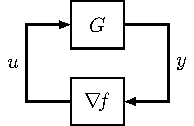
\includegraphics[width = .3 \textwidth]{text_figure1}
    \caption{Block diagram representation of iterative algorithms}
    \label{plot_block_diagram}
\end{figure}

Here, \(G\) represents the LTI system, while \(y\) and \(u\) are input and output of the gradient nonlinearity. For example, (FG) equation \eqref{eqn:FG} matches this representation if $u_k$ is defined as $\nabla f(y_k)$.
% can be rewritten to match this view as:
% \begin{subequations} \label{eqn:FG2}
% 	\begin{align}
% 	  x_{k+1}     &=x_k-\alpha u_k \label{eq_FGstate},       \\
% 	  y_{k+1} &=x_{k+1}+\beta (x_{k+1}-x_k), \label{eq_FGinterpolated point}, \\
% 	  u_k &= \nabla f(y_k) \label{eq_FGggradient}
% 	\end{align}
% \end{subequations}
The algorithm can then be put into state-space representation with augmented state $\xi _k = (x_k, x_{k-1})$ as:
\begin{subequations} \label{eqn:FGss }
	\begin{align}
	  \xi_{k+1} &= \bmat{(1+\beta) & -\beta\\ 1 & 0}\xi_k  + \bmat{-\alpha\\ 0}u_k \label{eq_FGssstate}, \\
	  y_k &= \bmat{1+\beta & \beta}\xi_k, \label{eq_FGssinterpolation},\\
	  u_k &= \nabla f(y_k) \label{eq_FGssgradient}
	\end{align}
\end{subequations}
in which function $f$ is $n$-multivariate, meaning  $x_k \in \mathbb{R}^{1\times n}$, $\xi_k \in \mathbb{R}^{2\times n}$, $y_k \in \mathbb{R}^{2\times n}$, $u_k \in \mathbb{R}^{2 \times n}$, and the gradient evaluation maps a row vector to a row vector $\nabla f:\mathbb{R}^{1\times n} \rightarrow \mathbb{R}^{1\times n}$.

The LTI system \(G\) can be expressed with four matrices that change in value depending on the algorithm and size depending on the number of past states used to update \(x\). For (GD), (FG), and (HB) as they are described in equations \eqref{eqn:GD}, \eqref{eqn:HB}, and \eqref{eqn:FG}, these matrices are:

\begin{table}[h!]
    \centering
	\scalebox{1.5}{%
    \begin{tabular}{c c c}
		GD & HB & FG \\
        \hline
        % Matrix 1
        $\left[\begin{array}{c|c}
            1 & -\alpha \\ \hline
            1 & 0 \\
        \end{array}\right] $
        &
        % Matrix 2
        $\left[\begin{array}{c c |c}
            1 + \beta & -\beta & -\alpha \\ 
			1 & 0 & 0 \\ \hline
            1 & 0 & 0 \\
        \end{array}\right] $
        &
        % Matrix 3
        $\left[\begin{array}{c c|c}
            1 + \beta & -\beta & -\alpha \\ 
			1 & 0 & 0 \\ \hline
            1 + \beta & -\beta & 0 \\
        \end{array}\right] $
        \\
    \end{tabular}}
\end{table}

Beyond the three listed examples, any other first-order methods can be transformed into an LTI system represented by state-space matrices, enabling the formulation of Lyapunov functions in the next sections and forming the first step at transforming the algorithm analysis problem into a convex semidefinite program.
% not only creates a representation easy to understand and operate on, but also in next sections enable the representation of the past states of an algorithm and the forming of a Lyapunov function.

\section{Interpolation condition} \label{constraint}
% \comment{Need some overview statement here. At a high level, what is meant by interpolation conditions?}
% \subsection*{Function class interpolation conditions}

In the field of robust control theory utilized by this Lyapunov-based approach, while an LTI system is relatively simple, the nonlinearity representing the gradient of the function cannot be efficiently solved. As a result, the Lyapunov-based approach replaces the nonlinearity with a characterization of the class of function. Since the algorithm is being analyzed at discrete iterates, the characterization of a function class can be done using interpolation conditions, a set of conditions on the nonlinearity's input $y$ and output $u$. Through this characterization, the block diagram representation is transformed into the block diagram depicted in Figure~\ref{plot_block_diagram2}.
\begin{figure}[h]
    \centering
	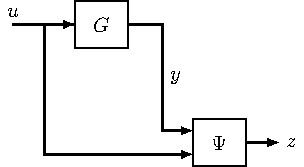
\includegraphics[width = .5 \textwidth]{text_figure2}
    \caption{Block diagram of iterative algorithms with gradient replaced by interpolation condition filter}
    \label{plot_block_diagram2}
\end{figure}
Here, the nonlinear gradient block is replaced with a filter or dynamical system $\Psi$. This dynamical system produces an output $z$ as some quadratic function of its inputs $y$ and $u$ before applying some constraint to the output $z$. Both the filter and its corresponding constraints depend on the properties of the gradient of the objective function, which are characterized by its \textit{interpolation conditions}. The interpolation conditions of a function class provide necessary and sufficient conditions under which there exists a function in that class that interpolates a given finite set of iterate-gradient pairs. These interpolation conditions depends on the characteristics of the function class. The analysis of any algorithm's performance at solving a function class is only possible if there exists interpolation conditions for that class.

While many function classes have interpolation conditions, this thesis and the Algorithm Analysis package focus on smooth strongly convex functions and their interpolation conditions, with the goal of analyzing the performance of algorithms at solving them, as many optmization problems such as linear regression or logistic regression in the machine learning field can be classified as convex optimization problems. This thesis uses the notation and definition of smooth strongly convex functions as \cite{tutorial}, which uses the notation $F_{m,L}$ and define the function class as continuously differentiable functions that satisfy:
\begin{enumerate}
	\item $L$-Lipschitz gradients: $\|\nabla f(x) - \nabla f(x)\| \leq L\|x-y\|$ for all $x, y \in \mathbb{R}$.
	\item $m$-strong convexity: $f(x) - \frac{m}{2}\|x\|^2$ is convex.
\end{enumerate}

The interpolation conditions for $L$-smooth and $m$-strongly convex functions was first formulated in \cite{taylor2016} and reformatted in \cite{tutorial} as:

\begin{theorem}[\cite{taylor2016}, Thm. 4; \cite{tutorial}, Thm. 3]
	\label{thm:interpolation_condition}
	Given index set \(I\), a set of triplets \(\{(y_k, u_k, f_k)\}_{k \in I}\) is $F_{m,L}$-interpolable, meaning there exists a function \(f \in F_{m,L}\) satisfying \(f(y_k) = f_k\) and \(\nabla f(y_k) = u_k\) if and only if
	\[
	 	2(L-m)(f_i - f_j) - mL\|y_i - y_j\|^2 + 2(y_i - y_j)^\tp (mu_i - Lu_j) - \|u_i - u_j\|^2 \geq 0
	\]
	for all $i,j\in I$.
\end{theorem}

As an example, if we define $x_0$ as the initial iterate of an algorithm optimization a 1 strong 10 smooth convex function (\(f \in \) \(F_{1,10}\)), $x_s$ as the minimizer, and only evaluate the gradient of $f$ at $x_k$ and $x_s$: $\nabla f(x_k)$ is the gradient of $f$ at $x_k$ and $\nabla f(x_s) = 0$ is the gradient of $f$ at $x_s$ (so $m=1$, $L=10$, and $I = \{s,k\}$), then the inequalities:
% \begin{equation} \label{eqn:int_cond}
% 	-20\|x_k\|^2 -20\|x_s\|^2 + 40\innerproduct{x_k}{x_s} + 22\innerproduct{\nabla f(x_k)}{x_k} - 22\innerproduct{\nabla f(x_k)}{x_s} - 2\|\nabla f(x_k)\|^2 \geq 0
% \end{equation}
% \begin{subequations} \label{eqn:Ly_ineq}
% 	\begin{align}
% 		18(f(x_0)-f(x_s))-10\|x_0\|^2 -10\|x_s\|^2 + 20\innerproduct{x_0}{x_s} + 2\innerproduct{\nabla f(x_0)}{x_0} - 2\innerproduct{\nabla f(x_0)}{x_s} - \|\nabla f(x_0)\|^2 &\geq 0      \\
% 		18(f(x_s)-f(x_0))-10\|x_0\|^2 -10\|x_s\|^2 + 20\innerproduct{x_s}{x_0} + 20\innerproduct{\nabla f(x_0)}{x_0} - 20\innerproduct{\nabla f(x_0)}{x_s} - \|\nabla f(x_0)\|^2 &\geq 0
% 	\end{align}
% \end{subequations}
\begin{equation} \label{eqn:int_cond}
	\begin{split}
		18(f(x_k)-f(x_s))-10\|x_k\|^2 -10\|x_s\|^2 + 20\innerproduct{x_k}{x_s} + 2\innerproduct{\nabla f(x_k)}{x_k} \\
		- 2\innerproduct{\nabla f(x_k)}{x_s} - \|\nabla f(x_k)\|^2 &\geq 0      \\
		18(f(x_s)-f(x_k))-10\|x_k\|^2 -10\|x_s\|^2 + 20\innerproduct{x_s}{x_k} + 20\innerproduct{\nabla f(x_k)}{x_k} \\
		- 20\innerproduct{\nabla f(x_k)}{x_s} - \|\nabla f(x_k)\|^2 &\geq 0
	\end{split}
\end{equation}
when satisfied interpolates $1$ strong $10$ smooth convex functions. Using interpolation condition, the gradient of any function belonging to the associated function class is represented with an inequality, one of the two components of the convex semidefinite problem needed to analyze algorithms.
% \begin{equation} \label{eqn:Gram}
% 	\bmat{\|y_i\|^2 & \innerproduct{y_j}{y_i} & \innerproduct{u_i}{y_i} \\ \innerproduct{y_i}{y_j} & \|y_j\|^2 & \innerproduct{u_i}{y_j} \\ \innerproduct{y_i}{u_i} & \innerproduct{y_j}{u_i} & \|u_i\|^2}
% \end{equation}
% \begin{equation} \label{eqn:int_cond2}
% 	% \begin{align}
% 	%   tr \bmat{y_i \\ y_j \\ u_i \\ u_j}^TH\bmat{y_i \\ y_j \\ u_i \\ u_j} + h^T\bmat{f_i \\ f_j} \geq 0 \\
% 	%   tr \bmat{y_i \\ y_j \\ u_i \\ u_j}^T\Lambda H\bmat{y_i \\ y_j \\ u_i \\ u_j} + \Lambda h^T\bmat{f_i \\ f_j} \geq 0 \\
% 	%   tr \Lambda \bmat{y_i \\ y_j \\ u_i \\ u_j}\bmat{y_i \\ y_j \\ u_i \\ u_j}^TH + \Lambda h^T\bmat{f_i \\ f_j} \geq 0
% 	\Lambda\bmat{-mL & 2mL & -mL & 2(m+L) & -2(m+L) & -2m}\bmat{||y_i||^2 \\ \innerproduct{y_i}{y_j} \\ ||y_j||^2 \\ \innerproduct{\nabla f(y_i)}{y_j} \\ \innerproduct{\nabla f(y_j)}{y_i} \\ ||\nabla f(y_j)||^2} \geq 0
% 	% \end{align}
% \end{equation}
% With $H = \bmat{-mL & mL & m & -L\\mL & -mL & -m & L\\m & -m & -1 & 1\\-L & L & 1 & -1}$ 
% %\in \Re^{6x6}%
% for all $\Lambda $ such that $\Lambda_{i,j} \geq 0$. Using this equation, \ref{eqn:int_cond} can be scaled by 10 and rewritten as: \label{eqn:int_cond3}
% \begin{equation} 
% 	\Lambda\bmat{-2 & 4 & -2 & 2.2 & -2.2 & -0.2}\bmat{||x_0||^2 \\ \innerproduct{x_0}{x_s} \\ ||x_s||^2 \\ \innerproduct{\nabla f(x_0)}{x_0} \\ \innerproduct{\nabla f(x_0)}{x_s} \\ ||\nabla f(x_0)||^2} \geq 0
% \end{equation}
% The constraints on $\Lambda $ are added to the optimization problem, and the resulting nonnegative inequalities \ref{eqn:int_cond2} are combined and used in the formulation of Lyapunov functions discussed in the next section.
% Whether an algorithm being analyzed uses the gradient of multiple past states to update, or the state-space representation of an algorithm include the gradient of more than one iterate, there might exists multiple iterate-gradient pairs, each creating an inequality for their interpolation. By combining these inequalities, each scaled by a nonnegative optimization variable $\lambda $, a tight representation of the function class can be created. The inequalities in \ref{eqn:int_cond} can be combined to create:
% Basing on this theorem, [\cite{tutorial}, Cor 4] presented a non-negative linear combination of inequalities to create a tight representation of the class of function, which can be rewritten in a way easier to implement into code as:
% \begin{corollary}[\cite{tutorial}, Cor. 4]
% 	Given a function \(f \in F_{m,L}\) and let \(y_k,...,y_{k-l}\) be a sequence of iterates; \(u_{k-i} = \nabla f(y_{k-i})\) and \(f_{k-i} = f(y_{k-i})\) for \(i \in 0,...l\). Then the inequality:
% 	holds for all \(\Lambda \in \mathbb{R}^{(l+2) * (l+2)}\) and \(\Lambda >= 0\), and \(\Pi(\Lambda)\) and  \(\pi(\Lambda)\) are defined as:
% \end{corollary}
\subsection*{Gram matrix interpolation condition}

It can be seen that other than the function values $f_i$ and $f_j$, the left hand side of the interpolation condition consists of the norm and inner product of the interpolated points and gradients. These elements create a Gram matrix of real-valued elements with which the interpolation can be defined as a function of. Theorem \ref{thm:interpolation_condition} can be transformed into:
\begin{equation} \label{eqn:condGram}
	% \trace[]\bmat{-mL & mL & m \\ mL & -mL & -m\\m & -m & -1}\bmat{||x0||^2 & \innerproduct{xs}{x0} & \innerproduct{\nabla f(x0)}{x0} \\ \innerproduct{x0}{xs} & ||xs||^2 & \innerproduct{\nabla f(x0)}{xs} \\ \innerproduct{x0}{\nabla f(x0)} & \innerproduct{xs}{\nabla f(x0)} & ||\nabla f(x0)||^2}] + 2(L-m)(f_i - f_j) \geq 0.
	\sum_{i,j\in I} \trace(\bmat{-mL & mL & m \\ mL & -mL & -m\\m & -m & -1}\bmat{\|y_i\|^2 & \innerproduct{y_j}{y_i} & \innerproduct{u_i}{y_i} \\ \innerproduct{y_i}{y_j} & \|y_j\|^2 & \innerproduct{u_i}{y_j} \\ \innerproduct{y_i}{u_i} & \innerproduct{y_j}{u_i} & \|u_i\|^2}) + 2(L-m)(f_i - f_j) \geq 0.
\end{equation}
for all $i,j\in I$. We can then define $[x; u]$ as the Gram matrix of a set of vectors representing every interpolated points, which is also every state and gradient an algorithm uses to update its iterate
% The performance measure and the left hand side of the interpolation conditions are formulated from the norm and inner products of the state vector the end point vector, with the Lyapunov function detailed in the next section formulated using the same elements along with the gradient of the function used by the algorithm. These expressions are elements of the Gram-matrix of the vector containing every expressions the algorithm uses to update the iterates and goal vector expression. For the interpolation condition \ref{eqn:int_cond2} and a gradient descent algorithm which derive the first iterate $x_1$ using the gradient at the initial state $x_0$, the Gram matrix is:

% \begin{equation} \label{eqn:trans_cond}
% 	\bmat{||x0||^2 & \innerproduct{xs}{x0} & \innerproduct{\nabla f(x0)}{x0} \\ \innerproduct{x0}{xs} & ||xs||^2 & \innerproduct{\nabla f(x0)}{xs} \\ \innerproduct{x0}{\nabla f(x0)} & \innerproduct{xs}{\nabla f(x0)} & ||\nabla f(x0)||^2}	\comment{.}
% \end{equation}

The elements of the Gram matrix are interpolable --- meaning there exists vectors the norm and inner product of which are elements of a Gram matrix --- if and only if the Gram matrix is positive semidefinite and the dimension $n$ of the state vectors to be greater than or equal to the rank of the Gram matrix. Since the problem classes the algorithm being analyzed is abstract, the Lyapunov-based approach makes the assumption that each function in every class has sufficiently large dimension. The other condition on the Gram matrix is applied is similar to those created from interpolation conditions and will also be used to construct the semidefinite problem. The constraint for the Gram matrix associated with \eqref{eqn:int_cond} is:
% \begin{equation} \label{eqn:trans_cond}
% 		\bmat{\|x_k\|^2 & \innerproduct{x_s}{x_k} & \innerproduct{\nabla f(x_k)}{x_k} \\ \innerproduct{x_k}{x_s} & \|x_s\|^2 & \innerproduct{\nabla f(x_k)}{x_s} \\ \innerproduct{x_k}{\nabla f(x_k)} & \innerproduct{xs}{\nabla f(x_k)} & \|\nabla f(x_k)\|^2} \succcurlyeq 0.
% 	\end{equation}

\begin{equation} \label{eqn:trans_cond}
	\bmat{\|x_i\|^2 & \innerproduct{x_j}{x_i} & \innerproduct{\nabla f(x_i)}{x_i} & \innerproduct{\nabla f(x_j)}{x_i}\\ \innerproduct{x_i}{x_j} & \|x_j\|^2 & \innerproduct{\nabla f(x_i)}{x_j} & \innerproduct{\nabla f(x_j)}{x_j} \\ \innerproduct{x_i}{\nabla f(x_i)} & \innerproduct{x_j}{\nabla f(x_i)} & \|\nabla f(x_i)\|^2 & \innerproduct{\nabla f(x_j)}{\nabla f(x_i)} \\ \innerproduct{x_i}{\nabla f(x_j)} & \innerproduct{x_j}{\nabla f(x_j)} & \innerproduct{\nabla f(x_i)}{\nabla f(x_j)} & \|\nabla f(x_j)\|^2} \succcurlyeq 0.
\end{equation}

% which is why we need to assume that the dimension is sufficiently large)}. This constraint is similar to those created from interpolation conditions and will also be used to construct the semidefinite problem.

\section{Lyapunov function derivation} \label{Lyapunov}
In the third and final step of the Lyapunov method, we:
\begin{enumerate}
	\item Use Lyapunov functions to represent the energy of the system.
	\item Apply conditions on the Lyapunov functions, whose satisfaction proves whether a performance rate can be guaranteed for the system.
	\item Formulate an optimization problem consisting of functions linear in the optimization variables, formed from the conditions on the Lyapunov functions and constraints created by the interpolation conditions. For any rate of performance, whether it can be guaranteed for the system depends on whether the optimization problem can be solved.
\end{enumerate}

The main goal of the program and the Lyapunov method it implement is to certify whether any given level of performance can be guaranteed, and uses \textit{convergence rate} as a measure of performance, which is defined as the rate at which the performance measure $\|x_k - x_s\|^2$ decreases after each iteration. This definition can be expressed in equation form as, given any $k \geq 0$ as the iterate of an algorithm and define $x_0$ as the initial iterate of the algorithm, a proven convergence rate guarantee of $\rho$ means:
\begin{equation} \label{eqn:convergence_rate}
	\|x_k - x_s\|^2 \leq \rho^k\|x_0 - x_s\|^2.
\end{equation}
%  In \cite{tutorial}, it is proven that a convergence rate can be guaranteed if there exist a $\lambda \geq 0$ and $P$ which makes the Lyapunov function nonpositive. Therefore, a minimum convergence rate can be guaranteed by solving for $P$ and $\lambda$ so that the Lyapunov function would satisfy 2 linear matrix inequalities. The mathematical basis of JuPE follows this approach with some modification. 

In the field of control, the Lyapunov function is a fundamental tool, defined as a nonnegative function that decreases in time along the orbit of a dynamical system and can be used to understand the behavior of a system. Under this definition, the dynamical system is the algorithm being analyzed, and two Lyapunov functions are used to certify whether or not a convergence rate can be guaranteed for a system. Consider the gradient descent algorithm and its representation in \eqref{eqn:GD}, define $\mathbf{x_k} = x_k - x_s$, the Lyapunov function takes the form:
% = \bmat{x_{k} - x_s \\ x_{k-1} - x_s}$, the Lyapunov function would take the form of:
\begin{equation}
	V(\mathbf{x}) = \trace(\mathbf{x_k}^TP\mathbf{x_k}) \label{eqn:Lyapunov}
\end{equation}
where $P$ is a symmetric matrix optimization variable. Note that the Lyapunov function represents a state of a system, in this case an algorithm, and for algorithms which update its iterate using multiple past states, $\mathbf{x_k}$ would have to include every states used to iterate. For example, for the Fast gradient algorithm as it is represented in \eqref{eqn:FG}, $\mathbf{x_k} = \bmat{x_{k} - x_s \\ x_{k-1} - x_s}$. Continuing the gradient descent example, if it is proven there exists some optimization variable $P$ so that Lyapunov functions satisfy the conditions:
\begin{subequations} \label{eqn:Ly_ineq}
	\begin{align}
	  \|x_k - x_s\|^2 - V(\mathbf{x_k}) \leq 0,      \\
	  V(\mathbf{x_{k+1}}) - \rho V(\mathbf{x_k}) \leq 0
	\end{align}
\end{subequations}
then the convergence rate of that algorithm is guaranteed to be faster than $\rho $ for every function in the function class. The first Lyapunov function inequality if satisfied guarantees for each iteration of an algorithm, the distance from the iterate to the minimizer $\|x_k - x_s\|^2$, which will be referred to in the rest of this thesis as the performance measure, is smaller or equal to the Lyapunov function. The second Lyapunov function inequality if satisfied guarantees after each iteration, the Lyapunov function decreases at a rate faster or equal to $\rho^2$ after each iteration. Together, if the optimization variable $P$ can be found so that the two inequalities are satisfied, a convergence rate of $\rho$ or faster can be guaranteed. This is proven in the proof of Lemma 5 of \cite{tutorial}, which can be modified to suit the gradient descent algorithm. For any $k \geq 0$:
\begin{equation}
	\|x_k - x_s\|^2 \leq V(\mathbf{x_{k}}) \leq \ldots \leq \rho^{k}V(\mathbf{x_{0}}) \leq \rho^k(C_0\|x_0 - x_s\|^2)
\end{equation}
where $C_0$ is a constant that depends on the intialization of the algorithm and the optimization parameter $P$.

The Lyapunov functions conditions in their current form cannot be proven, as they are quadratic functions of abstract state vectors. In order to find a variable $P$ that would satisfy these conditions using the Lyapunov method, we combine them with the left hand side of the constraints detailed in Section~\ref{constraint} and transform them into functions linear in the optimization variables.

Here, it can be seen that while these Lyapunov functions that are quadratic in $\mathbf{x_k}$, they are linear in the Gram matrix of the state and input vectors $[x_k, x_s, u_k]$. Define $I_n \in \mathbb{R}^{n \times n}$, the identity matrix with dimension $n$, the same as the dimension of the state vectors, the Lyapunov function can be transformed into:
% Define $\mathbf{e} = \bmat{1 & 1 & \ldots & 1}^\tp \in \mathbb{R}^n$ where $n$ is the dimension of $x_k$ and $x_s$, then the Lyapunov function inequalities can be transformed into:
\begin{subequations}  \label{eqn:Vx}
	\begin{align}
		V(\mathbf{x_k}) &= \trace[P(x_k - x_s)(x_k - x_s)^\tp]\\
					  &= \trace[\bmat{P &-P &0\\-P & P & 0\\0 & 0 & 0}\bmat{\|x_k\|^2 & \innerproduct{x_s}{x_k} & \innerproduct{u_k}{x_k} \\ \innerproduct{x_k}{x_s} & \|x_s\|^2 & \innerproduct{u_k}{x_s} \\ \innerproduct{x_k}{u_k} & \innerproduct{x_s}{u_k} & \|u_k\|^2}] \notag \\
		V(\mathbf{x_{k+1}}) &= \trace[P(x_{k+1} - x_s)(x_{k+1} - x_s)^\tp]\\
		&= \trace[P(Ax_k + Bu_k - x_s)(Ax_k + Bu_k - x_s)^\tp]\notag  \\
		&= \trace[P\bmat{A & B & -I_n}\bmat{x_k \\ u_k \\ x_s}\bmat{x_k \\ u_k \\ x_s}^\tp\bmat{A & B & -I_n}^\tp]\notag \\
		&= \trace[\bmat{A & B & -I_n}P\bmat{A & B & -I_n}^\tp\bmat{\|x_k\|^2 & \innerproduct{x_s}{x_k} & \innerproduct{u_k}{x_k} \\ \innerproduct{x_k}{x_s} & \|x_s\|^2 & \innerproduct{u_k}{x_s} \\ \innerproduct{x_k}{u_k} & \innerproduct{x_s}{u_k} & \|u_k\|^2}] \notag 
	\end{align}
\end{subequations}
while the performance measure $\|x_k - x_s\|^2$ can be transformed into:
\begin{equation}
	\|x_k - x_s\|^2 = \trace[\bmat{1 &-1 &0\\-1 & 1 & 0\\0 & 0 & 0}\bmat{\|x_k\|^2 & \innerproduct{x_s}{x_k} & \innerproduct{u_k}{x_k} \\ \innerproduct{x_k}{x_s} & \|x_s\|^2 & \innerproduct{u_k}{x_s} \\ \innerproduct{x_k}{u_k} & \innerproduct{x_s}{u_k} & \|u_k\|^2}].
\end{equation}
% &= \trace[\bmat{P_{1,1} & P_{1,2} & P_{2,1} & P_{2,2}}\bmat{||\xi_{k}||^2 & \innerproduct{\xi_{k}}{\xi_s} & \innerproduct{\xi_s}{\xi_{k}} & ||\xi_s||^2}^T]\\
		% V(\mathbf{x_{k+1}}) &= \trace[P(\xi_{k+1} - \xi_s)(\xi_{k+1} - \xi_s)^T]\\
		% 					&= \trace[\bmat{P_{1,1} & P_{1,2} & P_{2,1} & P_{2,2}}(A\xi_k + Bu_k -\xi_s)(A\xi_k + Bu_k -\xi_s)^T]\\
		% 					&= \trace[\bmat{P_{1,1} & P_{1,2} & P_{2,1} & P_{2,2}}\bmat{A||\xi_{k}||^2A^T \\ -\innerproduct{\xi_{k}}{\xi_s}A^T \\ -A\innerproduct{\xi_s}{\xi_{k}} \\ ||{\xi_s}||^2 \\ -\innerproduct{u_k}{\xi_s}B^T \\ -B\innerproduct{\xi_s}{u_k} \\
		% 					A\innerproduct{u_k}{\xi_{k}}B^T \\ B\innerproduct{\xi_{k}}{u_k}A^T \\ B||u_k||^2B^T}]
% note that the dimension of these simplifications makes sense as $\mathbf{x_k}$ is a $2\times n$ matrix, and the product $\mathbf{x_k}\mathbf{x_k}^T$ is a $2\times 2$ matrix. For gradient descent where the augmented state $\xi_k$ is just the state $x_k$, the Lyapunov function take the form of:
% \begin{subequations}  \label{eqn:Vx}
% 	\begin{align*}
% 		V(\mathbf{x_{k}}) = tr[(x_k - x_s)^TP(x_k - x_s)]\\
% 						  = tr[P(x_k - x_s)(x_k - x_s)^T]\\
% 						  = tr[P(x_kx_k^T - x_sx_k^T - x_kx_s^T + x_sx_s^T)] \\
% 						  = \bmat{P & -2P & P}\bmat{||x_k||^2 \\ \innerproduct{x_k}{x_s} \\ ||x_s||^2}
% 	\end{align*}
% \end{subequations}
% where $x_kx_s^T = x_sx_k^T = \innerproduct{x_k}{x_s}$. Similarly, $V(\mathbf{x_{k+1}})$ can be defined as:
% \begin{subequations}  \label{eqn:Vxp}
% 	\begin{align*}
% 		V(\mathbf{x_{k+1}}) = V(x_k - \alpha \nabla f(x_k)) \\
% 						  	= tr[(x_k - \alpha \nabla f(x_k) - x_s)^TP(x_k - \alpha \nabla f(x_k) - x_s]\\
% 						  	= tr[P(x_k - \alpha \nabla f(x_k) - x_s)(x_k - \alpha \nabla f(x_k) - x_s)^T]\\
% 						  	= \bmat{P & -2P & P & 2P\alpha & -2P\alpha & P\alpha^2}\bmat{||x_k||^2 \\ \innerproduct{x_k}{x_s} \\ ||x_s||^2 \\ \innerproduct{\nabla f(x_k)}{x_k} \\ \innerproduct{\nabla f(x_k)}{x_s} \\ ||\nabla f(x_k)||^2}
% 	\end{align*}
% \end{subequations}

% In the final step of the Lyapunov method, the Lyapunov functions are combined with the constraints derived from the interpolation conditions and linearized to form linear matrix inequalities. Finding the optimization variable that satisfies these inequalities is defined as a semidefinite problem, the solution to which proves whether a convergence rate can be guaranteed.

The Lyapunov functions $V(\mathbf{x_k})$ and $V(\mathbf{x_{k+1}})$, as well as the performance measure $\|x_k - x_s\|^2$ are linear functions of the Gram matrix and optimization variable P. This holds for every iterative gradient-based algorithm as they update using a linear function of past states $x$ and inputs $u$. If a different algorithm uses multiple iterates or multiple gradients to update, the corresponding Gram matrix of the Lyapunov functions will simple grow in dimension. Here, it should be noted that the Gram matrices in the Lyapunov functions are the same as those in the constraints, as every states and inputs in the vector set the Gram matrix is defined from have to be interpolated. However, each constraint include the function values $f_i, f_j$ on top of the elements of the Gram matrix present in the Lyapunov conditions. In order to combine the conditions in \eqref{eqn:Ly_ineq} with the constraints associated with the interpolation condtions, we first define the \textit{linear form} of both.

Define $[x; u]$ as a vector containing every elements of the Gram matrix and the function values at each interpolated points: The Lyapunov functions and each constraint are linear functions of $[x; u]$. In the gradient descent example, this vector is defined as:
\begin{equation} \label{eqn:xu}
	\bmat{x\\ u} = \bmat{\|x_k\|^2 \\ \innerproduct{x_s}{x_k} \\ \innerproduct{u_k}{x_k} \\ \innerproduct{x_k}{x_s} \\ \|x_s\|^2 \\ \innerproduct{u_k}{x_s} \\ \innerproduct{x_k}{u_k} \\ \innerproduct{x_s}{u_k} \\ \|u_k\|^2 \\ f(x_k) \\ f(x_s)}.
\end{equation}
The linear form of conditions on the Lyapunov functions $L1$ and $L2$ can be defined as:
\begin{subequations}
	\begin{align}
		\|x_k - x_s\|^2 - V(\mathbf{x_k}) = L1\bmat{x\\ u}\\
		V(\mathbf{x_{k+1}}) - \rho ^2V(\mathbf{x_k}) = L2\bmat{x\\ u}.
	\end{align}
\end{subequations}
For the constraints associated with the interpolation condtions, each is derived and scaled by a nonnegative obtimization variable $\Lambda$ before being combined with $L1$ and $L2$. For each constraint created by the interpolation conditions, an optimization variable $\Lambda $ is created and scaled with. The linear form of the constraints associated with the interpolation conditions \eqref{eqn:condGram} is:
\begin{equation} \label{eqn:constraints}
	\sum_{i \in C}M_i(\Lambda_i)\bmat{x\\u}
\end{equation}
where $C$ is the set containing every constraints created in \eqref{eqn:condGram} and \eqref{eqn:trans_cond} and $M_i$ is the linear form of each constraint scaled by a corresponding parameter $\Lambda _i$. The optimization parameters $\Lambda _i$ are constrained in the optimization problem to be nonnegative if it is a scalar, nonnegative element-wise if it is a vector, or positive semidefiinite if it is a matrix. When the constraints applied to these variables satisfied, equation \eqref{eqn:constraints} are nonnegative. At the same time, variables $\Lambda _i$ enable the solver to search for $\Lambda _i$ just as it does for $P$ so that the final linear function is satisfied. If the constraint is applied to a scalar variable in the case of those created by interpolation conditions associated with the function class, $M_i$ is the linear form of the scalar variable, or the left hand side of \eqref{eqn:int_cond} in the gradient descent example. On the other hand, if the constraint is applied to the Gram matrix, $M_i$ is the linear form of its trace. 

Lastly, as $L_1$, $L_2$ and $M_i(\Lambda_i)$ are all functions consisting of a vector or matrix of real-valued scalars and an optimization variable, we can combine them to create functions linear in the optimization variables, forming our optimization problem:
\begin{subequations} \label{eqn:LMI1}
	\begin{align} 
		L_1 + \sum_{i\in C} M_i(\Lambda_i^1) &= 0  \\
		L_2 + \sum_{i\in C} M_i(\Lambda_i^2) &= 0.
	\end{align}
\end{subequations}
For any convergence rate $\rho$, if some parameter $P$, $\Lambda_i^1$ and $\Lambda_i^2$ can be found which would solve the linear functions in \eqref{eqn:LMI1}, the Lyapunov function conditions specified in \eqref{eqn:Ly_ineq} is satisfied and that performance guarantee is feasible. However, if no such parameter can be found, the Lyapunov function conditions are not satisfied and the convergence rate cannot be guaranteed to be feasible. This can be proven as, for any $[x; u]$, \eqref{eqn:LMI1} can be multiplied with $[x; u]$. If the linear functions \eqref{eqn:LMI1} equal zero, and multiplying the linear form of the constraints by $[x; u]$ give us the interpolation conditions, which are constrained to be $\geq 0$, it must mean that $L1\bmat{x & u}^\tp$ is $\leq 0$:
\begin{subequations} \label{eqn:LMI2}
	\begin{align} 
		(L1 + \sum_{i\in C} M_i(\Lambda_i^1))\bmat{x & u}^\tp &= 0  \\
		\underbrace{L1\bmat{x & u}^\tp}_{\leq 0} + \underbrace{\sum_{i\in C} M_i(\Lambda_i^1)\bmat{x & u}^\tp}_{\geq 0} &= 0  \\
	\end{align}
\end{subequations}
and similarly, $L2\bmat{x & u}^\tp$ is $\leq 0$.
\begin{subequations} \label{eqn:LMI3}
	\begin{align*} 
		(L1 + \sum_{i\in C} M_i(\Lambda_i^1))\bmat{x & u}^\tp &= 0  \\
		\underbrace{L1\bmat{x & u}^\tp}_{\leq 0} + \underbrace{\sum_{i\in C} M_i(\Lambda_i^1)\bmat{x & u}^\tp}_{\geq 0} &= 0  \\
		(L2 + \sum_{i\in C} M_i(\Lambda_i^1))\bmat{x & u}^\tp &= 0  \\
		\underbrace{L2\bmat{x & u}^\tp}_{\leq 0} + \underbrace{\sum_{i\in C} M_i(\Lambda_i^1)\bmat{x & u}^\tp}_{\geq 0} &= 0  \\.
	\end{align*}
\end{subequations}
Together, $L1\bmat{x & u}^\tp \leq 0$ and $L2\bmat{x & u}^\tp \leq 0$ form the conditions on the Lyapunov functions, and if \eqref{eqn:LMI1} is solved, it means that the convergence rate is feasible.

Since we know how to certify whether a convergence rate guarantee is feasible, the worst-case performance of the system or fastest convergence rate that can be guaranteed for said system can be found by performing bisection search for the smallest value $\rho$ between 0 and 1 with which the optimization problem is feasible within some margin of error.
% Both components of the LMIs, the Lyapunov functions and the left hand side of the interpolation conditions constraints, are formulated from the norm and inner products of the state vector the end point vector. These expressions are elements of the Gram-matrix of the vector containing every expressions the algorithm uses to update the iterates and goal vector expression. For any algorithm which updates the first iterate $x_1$ using the gradient at the initial state $x_0$, the Gram matrix is:
% \begin{equation} \label{eqn:trans_cond}
% 	\bmat{||x0||^2 & \innerproduct{xs}{x0} & \innerproduct{\nabla f(x0)}{x0} \\ \innerproduct{x0}{xs} & ||xs||^2 & \innerproduct{\nabla f(x0)}{xs} \\ \innerproduct{x0}{\nabla f(x0)} & \innerproduct{xs}{\nabla f(x0)} & ||\nabla f(x0)||^2]}	
% \end{equation}
% The linear matrix inequalities can now be completed by adding the constraints created by function class and transpose interpolation conditions. These constraints similar to the Lyapunov functions are linear functions of the Gram matrix. Using the transformation shown in \ref{eqn:condGram}, inequality \ref{eqn:int_cond} takes the form:
% \begin{equation} \label{eqn:int_cond_Gram}
% 	\trace[\bmat{-20 & 20 & 20 \\ 20 & -20 & -2\\2 & -20 & -2}\bmat{\|x_k\|^2 & \innerproduct{x_s}{x_k} & \innerproduct{\nabla f(x_k)}{x_k} \\ \innerproduct{x_k}{x_s} & \|x_s\|^2 & \innerproduct{\nabla f(x_k)}{x_s} \\ \innerproduct{x_k}{\nabla f(x_k)} & \innerproduct{x_s}{\nabla f(x_k)} & \|\nabla f(x_k)\|^2}] \geq 0.
% \end{equation}
%  Adding equation \ref{eqn:int_cond_Gram} to equations \ref{eqn:LMI1}, we derive the final linear matrix inequality. Solving this semidefinite program certifies the convergence rate of an algorithm with state-space matrices A and B and that uses 1 past state to iterate at optimizing $10$-smooth and $1$-strongly convex functions:
% \begin{subequations}
% 	\begin{align*} \label{eqn:LMI2}
% 		\bmat{1 &-1 &0\\-1 & 1 & 0\\0 & 0 & 0} - \bmat{P &-P &0\\-P & P & 0\\0 & 0 & 0} + \Lambda \bmat{-20 & 20 & 20 \\ 20 & -20 & -2\\2 & -20 & -2} == 0\\
% 		\bmat{A & B & -\mathbf{e}}P\bmat{A & B & -\mathbf{e}}^\tp - \bmat{P &-P &0\\-P & P & 0\\0 & 0 & 0}  + \Lambda \bmat{-20 & 20 & 20 \\ 20 & -20 & -2\\2 & -20 & -2} == 0\\
% 	\end{align*}
% \end{subequations}
% The elements of the Gram matrix are interpolable - meaning there exists vectors $x0$, $x_s$ and $\nabla f(x0)$ with which they exists, if and only if the Gram matrix is positive semidefinite. This constraint similar to those created by the interpolation condition are scaled by an optimization variable $\Lambda$ to create the constraint:
% \begin{equation} \label{eqn:trans_cond}
% 	\Lambda\bmat{||x0||^2 & \innerproduct{xs}{x0} & \innerproduct{\nabla f(x0)}{x0} \\ \innerproduct{x0}{xs} & ||xs||^2 & \innerproduct{\nabla f(x0)}{xs} \\ \innerproduct{x0}{\nabla f(x0)} & \innerproduct{xs}{\nabla f(x0)} & ||\nabla f(x0)||^2]} \geq 0
% \end{equation}
% The convex SDP can now be completed with the addition the constraints created by function class' interpolation condition and the constraints on the Gram matrix. By scaling each constraint added to the Lyapunov functions by an optimization variable $\Lambda$, the solver can search for $\Lambda$ just as it does for $P$ so that the linear matrix inequality is satisfied. For each constraint $\Lambda $ is constrained in the optimization problem to be nonnegative if the left hand side of the constraint is a scalar, nonnegative element-wise if it is a vector, or positive semidefiinite if it is a matrix. The left hand side of the scaled constraints are then combined with the Lyapunov functions to create the final linear matrix inequality. For the gradient descent example, using the initial state $x_0$ to replace the state used to update $x_k$ in \ref{eqn:Vx} and \ref{eqn:Vxp}, the LMI is:
% \begin{subequations} \label{eqn:Ly_ineq2}
% 	\begin{align*}
% 		\bmat{1-P-2\Lambda \\ -2+2P+4\Lambda \\ 1-P-2\Lambda \\ 2.2\Lambda \\ -2.2\Lambda \\ -0.2\Lambda}^T\bmat{||x_k||^2 \\ \innerproduct{x_k}{x_s} \\ ||x_s||^2 \\ \innerproduct{\nabla f(x_k)}{x_k} \\ \innerproduct{\nabla f(x_k)}{x_s} \\ ||\nabla f(x_k)||^2} + \Lambda tr(\bmat{||x0||^2 & \innerproduct{xs}{x0} & \innerproduct{\nabla f(x0)}{x0} \\ \innerproduct{x0}{xs} & ||xs||^2 & \innerproduct{\nabla f(x0)}{xs} \\ \innerproduct{x0}{\nabla f(x0)} & \innerproduct{xs}{\nabla f(x0)} & ||\nabla f(x0)||^2]}) \leq 0 \\
% 		\bmat{P-P\rho^2-2\Lambda \\ -2P+2P\rho^2+4\Lambda \\ P-P\rho^2-2\Lambda \\ 2P\alpha+2.2\Lambda \\ -2P\alpha-2.2\Lambda \\ P\alpha^2-0.2\Lambda}^T\bmat{||x_k||^2 \\ \innerproduct{x_k}{x_s} \\ ||x_s||^2 \\ \innerproduct{\nabla f(x_k)}{x_k} \\ \innerproduct{\nabla f(x_k)}{x_s} \\ ||\nabla f(x_k)||^2} + \Lambda tr(\bmat{||x0||^2 & \innerproduct{xs}{x0} & \innerproduct{\nabla f(x0)}{x0} \\ \innerproduct{x0}{xs} & ||xs||^2 & \innerproduct{\nabla f(x0)}{xs} \\ \innerproduct{x0}{\nabla f(x0)} & \innerproduct{xs}{\nabla f(x0)} & ||\nabla f(x0)||^2]}	)\leq 0
% 	\end{align*}
% \end{subequations}
% \comment{From these equations, it is not exactly clear how this is a linear matrix inequality. Here, quantities such as $\|x_k\|^2$ are not considered as a variable in $x_k$, but are themselves scalar variables in the analysis. Moreover, these are \textit{algorithm variables}, not \textit{optimization variables} (the optimization variables are $P$ and $\Lambda$). Each of the above expressions is written as a linear function of the optimization variables using the \texttt{linearform} method in Julia, and then this linear function is set equal to zero.}
% The optimization problem can now be solved for any convergence rate $\rho$ whether there exist $P$ and $\Lambda $ so that the inequality are satisfied, proving whether $\rho$ can be guaranteed. The smallest convergence rate guarantee can be found by performing bisection search for the smallest value $\rho$ between 0 and 1 with which the optimization problem is feasible.
% By expanding \ref{eqn:xTPx}, we can see that $\mathbf{x}^T\mathbf{x}$ is a linear function of real variable, which can be transformed into a linear form. For example, for a gradient descent algorithm with step size $\alpha $ and $\xi _{k+1} - \xi _s = \bmat{x_k - \alpha * \nabla f(x_k) - x_s \\ x_k - x_s}$, we can define $o = \bmat{||x_k||^2 \\ <x_k, x_s> \\ ||x_s|| \\ ||\nabla f(x_k)||^2 \\ <\nabla f(x_k), x_k> \\ <\nabla f(x_k), x_s>}$ and $\mathbf{X}$ and $\mathbf{X^+}$as:
% \begin{subequations}  \label{eqn:X}
% 	\begin{gather}
% 		\mathbf{X}^T*o	= (\xi _k - \xi _s)^T*P*(\xi _k - \xi _s) \\
% 		\mathbf{X} = \bmat{1 & 0 & 0 & 0 & 0 & 0 \\ 0 & 1 & 0 & 0 & 0 & 0 \\ 0 & 0 & 1 & 0 & 0 & 0 \\ 0 & 0 & 0 & 0 & 0 & 0 \\ 0 & 0 & 0 & 0 & 0 & 0 \\ 0 & 0 & 0 & 0 & 0 & 0} \\
% 		\mathbf{X^+} = \bmat{1 & 0 & 0 & 0 & 0 & 0 \\ 0 & 1 & 0 & 0 & 0 & 0 \\ 0 & 0 & 1 & 0 & 0 & 0 \\ 0 & 0 & 0 & -\alpha ^2 & 0 & 0 \\ 0 & 0 & 0 & 0 & -2\alpha & 0 \\ 0 & 0 & 0 & 0 & 0 & -2\alpha}
% 	\end{gather}
% \end{subequations}
% Through this transformation, the updated state can be expressed is a linear function of $\mathbf{X}$ for any algorithm $\mathbf{X^+} = A\mathbf{X}$ where A is a real matrix. Similarly, $||\xi _k - \xi _s||^2$ can also be transformed into linear form $\mathcal{P} $ so that $\mathcal{P}^T*o = ||\xi _k - \xi _s||^2$. \ref{eqn:Ly_ineq} can now be transformed into:
% \begin{subequations} \label{eqn:newLy_ineq}
% 	\begin{align}
% 	  \mathcal{P} - tr(\mathbf{X}^TP) \leq 0      \\
% 	  tr(\mathbf{X}(A^TPA- \rho ^2P)) \leq 0
% 	\end{align}
% \end{subequations}
% \begin{equation} \label{eqn:Lyapunov}
% 	V(x) = <P, X[x; u]> = <X^T P, [x; u]>
% \end{equation}